\documentclass{article}

\usepackage{amsmath}
\usepackage{graphicx}

\begin{document}

In Appendix A, the first unnumbered equation is

\begin{equation}
      {d^2\sigma \over d\Omega dE_\gamma}
\end{equation}
which is equivalent to 
\begin{equation}
      {d^3\sigma \over d\cos\theta d\phi E_\gamma}
\end{equation}.

\begin{equation}
  \Delta\sigma^{i,j,k} = \int^{E_i}_{E_{i-1}}\int^{\theta_j}_{\theta_{j-1}}\int^{\phi_k}_{\phi_{k-1}} {d^2\sigma \over d\cos\theta dE_\gamma}dE_\gamma \sin\theta d\theta d\phi
  \tag{A1[sic]}
\end{equation}
Eq. (A1) is internally inconsistent. Cross section should be differential in $\phi$. Limits of integration for $\theta$ should be those for $\cos\theta$. I.e.,
\begin{equation}\Delta\sigma^{i,j,k} = \int^{E_i}_{E_{i-1}}\int^{\cos\theta_j}_{\cos\theta_{j-1}}\int^{\phi_k}_{\phi_{k-1}} {d^3\sigma \over d\cos\theta d\phi dE_\gamma}dE_\gamma d\cos\theta d\phi\end{equation}
and since
\begin{equation}{d\cos\theta \over d\theta} = -\sin\theta\end{equation}
we get
\begin{equation} d\Omega = d\cos\theta d\phi = -\sin\theta d\theta d\phi \end{equation}

(A1) becomes

\begin{equation}\Delta\sigma^{i,j,k} = \int^{E_i}_{E_{i-1}}\int_{\theta_j}^{\theta_{j-1}}\int^{\phi_k}_{\phi_{k-1}} {d^3\sigma \over \sin\theta d\theta d\phi dE_\gamma} dE_\gamma \sin\theta d\theta d\phi\end{equation}

or

\begin{equation}\Delta\sigma^{i,j,k} = \int^{E_i}_{E_{i-1}}\int_{\theta_j}^{\theta_{j-1}}\int^{\phi_k}_{\phi_{k-1}} {d^2\sigma \over d\Omega dE_\gamma} dE_\gamma \sin\theta d\theta d\phi\end{equation}

or

\begin{equation}\Delta\sigma^{i,j,k} = \int^{E_i}_{E_{i-1}}\int_{\theta_{j-1}}^{\theta_j}\int^{\phi_k}_{\phi_{k-1}} {d^3\sigma \over d\theta d\phi dE_\gamma} dE_\gamma d\theta d\phi\end{equation}

as one might expect.

We introduce and ``observed'' cross section where detector efficiency $\epsilon(E_\gamma,\theta,\phi)$ is taken into account.
\begin{equation}
\Delta\sigma^{i,j,k}_{\rm obs} = \int^{E_i}_{E_{i-1}}\int_{\theta_{j-1}}^{\theta_j}\int^{\phi_k}_{\phi_{k-1}} \epsilon(E_\gamma,\theta,\phi) {d^3\sigma \over d\theta d\phi dE_\gamma} dE_\gamma d\theta
\end{equation}
and introduce the observed cross section in a bin of energy and polar angle per unit azimulthal angle
\begin{equation}
\Delta\sigma^{i,j}_{\rm obs}(\phi) \approx {\Delta\sigma^{i,j,k}_{\rm obs} \over \phi_k - \phi_{k-1}} \approx \int^{E_i}_{E_{i-1}}\int_{\theta_{j-1}}^{\theta_j} \epsilon(E_\gamma,\theta,\phi) {d^3\sigma \over d\theta d\phi dE_\gamma} dE_\gamma d\theta\end{equation}

The probability of scattering is $p = \sigma/A$ where $\sigma$ is the total cross section for scattering, $A$ is the nominal area where scattering can occur. Let us call $N_t$ the number of target particles and $N_\gamma$ the number of beam particles. $N_t = \rho AL$ where $\rho$ is then target number volume density and $L$ is the length of the target. The number of scattering events $N_s$ is then
\begin{equation}
N_s = N_\gamma N_t p = N_\gamma(\rho A L){\sigma\over A} = N_\gamma\rho L\sigma
\end{equation}

If we define the yield $Y$ as the number of detected scattering events, then $Y = \epsilon N_s$ where $\epsilon$ is the detection efficiency. So
\begin{equation}
Y = N_\gamma\rho L\sigma\epsilon
\end{equation}
which recovers eq.~(A2). The yield on one bin is
\begin{equation}
Y^{i,j,k} \approx N^i_\gamma\rho L\Delta\sigma^{i,j,k}\epsilon^{i,j,k} \\
\approx N^i_\gamma\rho L\Delta\sigma^{i,j,k}_{\rm obs}
\end{equation}
Define the yield per unit $\phi$ interval in the $i$th energy bin and $j$th theta bin
\begin{equation}
Y^{i,j}(\phi) = N^i_\gamma\rho L\Delta\sigma^{i,j}_{\rm obs}(\phi)
\end{equation}
where we have made the approximation that $\epsilon^{i,j,k} \approx \epsilon(E_\gamma,\theta,\phi)$

In eq.~(A5) all cross sections are measured for the same target. Flux and target density is eliminated by definition of cross section.

\begin{equation}
{d\sigma_\perp \over d\Omega} = {d\sigma_a \over d\Omega}[1+P_\perp\Sigma\cos 2\phi] \tag{A3} \\
\end{equation}
\begin{equation}
{d\sigma_\parallel \over d\Omega} = {d\sigma_a \over d\Omega}[1-P_\parallel\Sigma\cos 2\phi] \tag{A4} \\
\end{equation}

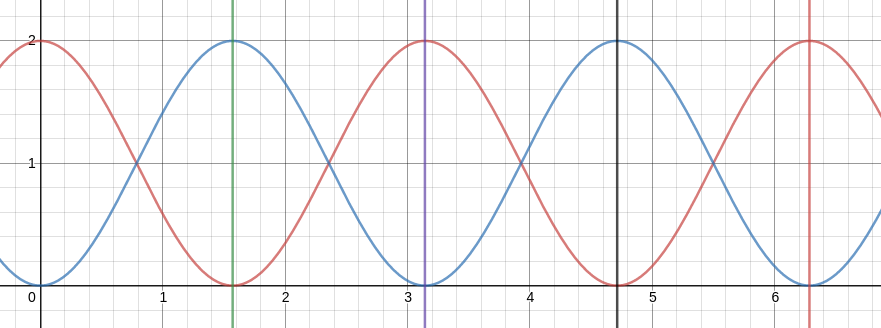
\includegraphics[width=4in]{assymetry.png}

\begin{equation}
{d\sigma_a \over d\Omega} = {1 \over 2} \left( {d\sigma_\perp \over d\Omega} + {d\sigma_\parallel \over d\Omega} \right) \tag{A5} \\
\end{equation}

Polarization $P$ is a function of energy. Analyzing power $\Sigma$ is a function of energy and polar angle. So we could write

\begin{equation}
{d^3\sigma^{i,j}_\perp \over dE_\gamma d\theta d\phi} = {d^3\sigma^{i,j}_a \over dE_\gamma d\theta d\phi}[1+P^i_\perp\Sigma^{i,j}\cos 2\phi] \\
\end{equation}
\begin{equation}
{d^3\sigma^{i,j}_\parallel \over dE_\gamma d\theta d\phi} = {d^3\sigma^{i,j}_a \over dE_\gamma d\theta d\phi}[1+P^i_\parallel\Sigma^{i,j}\cos 2\phi] \\
\end{equation}
\begin{equation}
  {d^3\sigma^{i,j}_a \over dE_\gamma d\theta d\phi}
  = {1 \over 2} \left( {d^3\sigma^{i,j}_\perp \over dE_\gamma d\theta d\phi}
  + {d^3\sigma^{i,j}_\parallel \over dE_\gamma d\theta d\phi} \right)
\end{equation}

\begin{equation}
  \begin{split}
f^{i,j}(\phi) & = \rho L\int^{E_i}_{E_{i-1}}\int_{\theta_{j-1}}^{\theta_j} \epsilon(E_\gamma,\theta,\phi) {d^2\sigma \over d\Omega dE_\gamma} dE_\gamma \sin\theta d\theta \\
& = \rho L\int^{E_i}_{E_{i-1}}\int_{\theta_{j-1}}^{\theta_j} \epsilon(E_\gamma,\theta,\phi) {d^3\sigma \over d\theta d\phi dE_\gamma} dE_\gamma d\theta \\
& {\rm and} \\
& \tilde Y^{i,j}(\phi) = {Y^{i,j}(\phi) \over N^i_\gamma}
\end{split} \tag{A6}
\end{equation}

There are three $f^{i,j}(\phi)$s, $f_a$, $f_\perp$, and $f_\parallel$ where the differential cross section for each type is substituted into (A6). They are the normalized yield in bin $i,j$ per unit azimuthal angle. So
\begin{equation}
  \begin{split}
    \tilde Y^{i,j}(\phi) & = \rho L\Delta\sigma^{i,j}_{\rm obs}(\phi) \\
    & = \rho L\int^{E_i}_{E_{i-1}}\int_{\theta_{j-1}}^{\theta_j} \epsilon(E_\gamma,\theta,\phi) {d^3\sigma \over d\theta d\phi dE_\gamma} dE_\gamma d\theta \\
    & = f^{i,j}(\phi)
  \end{split}
\end{equation}
What? $\tilde Y^{i,j}(\phi)$ and $f^{i,j}(\phi)$ are the same thing?

We make the identity

\begin{equation}
  f^{i,j}_a(\phi) = f^{i,j}(\phi)
\end{equation}

Note that $f^{i,j}_a(\phi)$ is never defined in the paper.

\begin{equation}
  \tilde Y^{i,j}_a = \int^{2\pi}_0 f^{i,j}_a(\phi)d\phi
  \tag{A7}
\end{equation}

\begin{equation}
  \tilde Y^{i,j}_\perp = \int^{2\pi}_0 f^{i,j}_a(\phi)[1+P^i_\perp\Sigma^{i,j}\cos2\phi]d\phi
  \tag{A8}
\end{equation}

\begin{equation}
  \tilde Y^{i,j}_\parallel = \int^{2\pi}_0 f^{i,j}_a(\phi)[1-P^i_\parallel\Sigma^{i,j}\cos2\phi]d\phi
  \tag{A9}
\end{equation}

\end{document}

